\chapter{Background and Related Work\label{chap:relatedWork}}
    This chapter outlines the necessary background knowledge needed for this work in Section \ref{sec:background}, then all related work is listed in Section \ref{sec:relatedWork}.
    
\section{Background} \label{sec:background}
    \Edited{Added intro paragraph}
    In this section we first introduce GitHub and Stack Overflow in Section~\ref{background:GH_SO} as the two most popular collaborative platforms in software engineering. In Section~\ref{background:text_processing} we outline the best practises of pre-processing textual data containing software artifacts. Section~\ref{LDA_bestPractises} will introduce topic modeling, and we will offer a lengthy background on LDA models. Background will conclude with a brief introduction of all evaluation metrics used throughout the thesis in Section~\ref{background:metrics}.
    
    \subsection{GitHub and Stack Overflow\label{background:GH_SO}}
        \Edited{Adding intro about GH}
        GitHub (GH) is the most popular social coding platform that allows massive worldwide collaboration for software developers on open source projects. In 2018 it was reported that GitHub had a total of more than 100 million repositories \cite{johnson_2018}, but search results from March 2020 indicate only over 28,6 million repositories are public\footnote{\url{https://github.com/search?q=is:public}}. As of March 2020, GitHub search results report over 37,7 million users\footnote{\url{https://github.com/search?q=type:user&type=Users}}. As early as 2014 GitHub was already called \emph{`the largest code hosting website in the world'} by Gousios et al. \cite{gousios2014lean}. GitHub also reported that 10 million new users joined in 2019. What is even more incredible that a total of 1.7 million students have learned to code on GitHub in 2019, which is 55\% more than in the previous year \cite{octoverse_2019}. These statistics clearly show how important GitHub is for the software development process. Hauff and Gousios \cite{hauff2015matching} mentioned that a developer's GitHub profile could become of interest to potential employers and recruiters, as they could learn more about a candidate's skills and interests. 
    
        Stack Overflow (SO) is the most popular question answering website for software developers, providing a large amount of code snippets and free-form text on a wide variety of topics. In a recent public data dump from December 9th 2018~\footnote{\url{https://zenodo.org/record/2273117}}, SO listed over 42 million posts from almost 10 million registered users. Similar to other software artifacts such as source code files and documentation, text and code snippets on SO evolve over time. An example of this is when the SO community fixes bugs in code snippets, clarifies questions and answers, and updates documentation to match new API versions. Studying Stack Overflow, its posts, users, and trends will shed some light on the evolution of expertise in such software artifacts. Furthermore, mining Stack Overflow has been a very popular research topic in Software Engineering over the past few years, thus Section~\ref{RW:mining_GH_SO}
        
    \subsection{Text Processing of Software Engineering Data \label{background:text_processing}}
        Textual data on Stack Overflow and GitHub contains a large variety of domain-specific (i.e., software engineering) terminology mixed with source code. Stack Overflow posts contain rich software artifacts such as code snippets, text blocks explaining problems and solutions using text and source code, comments which can be associated with a question or an answer, and hyperlinks to references such as API documentation or a publication explaining an answer. Liao et al. \cite{liao2019status} in their study on GitHub mention that developers on GitHub debate ``project bugs, enhancements, and tasks in issue discussions''. The authors stated that a text corpus built on GitHub data is most likely to contain
        code snippets, error messages and warnings, technical jargon and casual natural language, which theoretically should reveal someone's expertise.
        
        We can conclude that textual data on both GitHub and Stack Overflow captures a variety of aspects of software development, but its technical terminologies, mix of text and source code makes it difficult to extract the proper textual data to be analyzed. When performing text pre-processing on both sources of data, we need to find the right balance between more than a dozen pre-processing techniques in order to clean up the data just the right way, without removing software engineering domain-specific words and damaging the contextual details of software artifacts. Deciding on a precise set of techniques for the pre-processing routine can be a challenging task, thus we conducted an extensive research on what text pre-processing techniques have been previously used for analyzing GitHub and Stack Overflow data.
        
        Tian et al. \cite{tian2013predicting} pre-processed textual data by performing tokenization, stop-word removal and stemming. They also split function names from cleaned up source code related keywords in the text processing phase.
        
        Campbell et al. have also addressed the challenge of data pre-processing. In their
        book chapter~\cite{campbell2015latent} on extracting topics from software engineering data, they say that generally those who use LDA apply the following pre-processing steps: perform lexical analysis, optionally remove stop words and performing stemming, then build vocabulary, optionally filter out uncommon and frequently used words, and lastly create a bag-of-words representation of text.
        
        Treude and Wagner \cite{treude2019predicting} have performed similar but separate pre-processing routines on Stack Overflow and GitHub data. Their Stack Overflow data cleaning routine consists of removing line breaks, code blocks, all HTML tags, replacing HTML symbols and strings indicating special characters with their corresponding character, and replacing sequences of white-space with a single space. Their GitHub pre-processing routine is the same as the Stack Overflow data cleaning routine, with a few extra steps, such as removing vertical and horizontal lines, code comments, characters denoting sections headers, characters that indicate formatting or links. 
        
        Efstathiou et al. \cite{efstathiou2018word} converted text from Stack Overflow into lowercase, removed code snippets and HTML tags, then performed a ``conservative punctuation removal, keeping symbols that often appear in programming commands, such as ``+'' and ``\#'' which are essential for differentiating ``C'', ``C++'', and ``C\#'' from one another''. 
        
        Boyd-Graber et al.'s book chapter~\cite{boyd2014care} recommends HTML symbol and stopword removal, then normalizing strings by converting to lower case and applying any kind of stemming algorithm, then applying tokenization and any kind of phrase detection algorithm as the proper pre-processing routine before fitting topic models on textual data.
        
        Liao et al. \cite{liao2019status} analyzed issue discussions on GitHub, and in their pre-processing steps they filtered out code-specific language, which was enclosed in HTML tags. The authors then removed short posts contained less than five tokens and distinguished between data generated by developers who never committed code to a project, and those who did.
    
    \subsection{Topic Modeling\label{LDA_bestPractises}}
        
        Topic modeling is a technique used in the field of text mining to discover hidden patterns in a collection of textual documents. These hidden patterns are called \emph{topics} and they can be modeled using distributions. A \emph{topic} can be defined as a collection of co-occurring words that have been grouped together by a topic modeling algorithm.
        
        Topic models are highly popular unsupervised statistical models in machine learning, as they provide a way to find structure in unstructured textual data. The most popular use case scenarios for topic models are text clustering and information retrieval tasks, where the goal is to discover structure and extract insight from text documents. Examples of such application could be the use of topic modeling to group similar words into topics, thus, forming text clusters. Another sample application could be using topic modeling to detect trends in online documents and help building a recommender system for users to find similar online content. 
        
        The most used topic modeling algorithms are Latent Dirichlet Allocation (\emph{LDA}), Latent Semantic Indexing (\emph{LSI}) and Non-Negative Matrix Factorization (\emph{NMF}). The focus of this section will be on \emph{LDA} models.
    
        \subsubsection{What is an LDA model?}
            
           LDA is a generative probabilistic Bayesian topic model. This means that LDA observes probability distributions in input data and generates topics based on an underlying distribution of the latent (hidden) variables. LDA being also a Bayesian model, it allows Bayesian inference methods to be performed on the model. LDA models need as input a collection of documents in the form of a \emph{Document-Term Matrix} containing the number of occurrences of each word $j$ in each document $i$, and a few hyper-parameters. 
           
           LDA models come with assumptions. The first assumption is that each input document has multiple topics. This is also referred to as mixtures of topics. Furthermore, each document can be modeled as a discrete probability distribution over some number of latent (hidden) topics. The second assumption is that a topic is a collection of words with a discrete probability distribution over all unique words contained in the input documents, which is also referred to as a vocabulary of words. Lastly, the third assumption is that the number of topics is fixed and needs to be specified by the user, as LDA models do not have the capability to infer the number of topics from the input collection of documents.
           
            A trained LDA model outputs two matrices: \emph{Topic Document Matrix} and \emph{Term Topic Matrix}. The \emph{Topic Document Matrix} contains probabilities of each document generating a specific topic. The \emph{Term Topic Matrix} contains probabilities of each topic generating a specific word from the vocabulary. These two matrices can be further processed and transformed into a weighted list of topics representing every document. Furthermore, each topic contains a list of words, which describes the topic. Large collections of unstructured textual data can be summarized, clustered, linked and even pre-processed using a LDA model and its rich output \cite{campbell2015latent}.
        
        \subsubsection{How does an LDA model work?}
        
            Apart from input collection of documents, LDA has four parameters:
            
            \begin{enumerate}
                \item $\alpha$ represents a document's prior topic distribution, and it is sampled randomly from a Dirichlet distribution with $\alpha$ hyper-parameter. This parameter is also referred to as the prior document-topic density. Larger values of $\alpha$ result in documents containing more topics, while smaller values of $\alpha$ result in documents containing less topics. 
                
                \item $\beta$ represents a topic's prior word distribution, and it is sampled randomly from a Dirichlet distribution with $\beta$ hyper-parameter. This parameter is also referred to as the prior topic-word density. Larger values of $\beta$ result in topics containing a larger number of words from the corpus, while lower values of $\beta$ result in topics containing less words from the corpus.
                
                \item $K$ represents the number of topics to be extracted from the input collection of documents.
                
                \item The number of iterations represents the maximum number of iterations allowed for the LDA algorithm to convergence.
            \end{enumerate}
        
            LDA assumes that it receives a collection of $D$ documents, each of length $L_i$ as input. Being a generative probabilistic model, LDA has a generative process, which can be described in the following steps:
            
            \begin{enumerate}
                \item For each topic $k$ in \{1, ..., $K$\} draw a word distribution $\phi_k \sim Dir(\beta)$
                \item For each document $d$ in \{1, ..., $D$\} draw a topic distribution $\phi_d \sim Dir(\alpha)$
                \item For each word $i$ of document $d$ draw a topic distribution $z_{d,i} \sim Multinomial(\phi_d)$ and a word distribution $w_{d,i} \sim Multinomial(\phi_{z_{d,i}})$
            \end{enumerate}
            
            \begin{figure}[!ht]
              \centering
              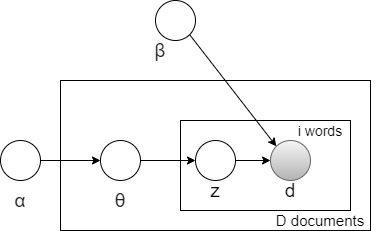
\includegraphics[width=0.7\textwidth]{figures/LDA_graphical.jpg}\\
              \caption{Graphical representation of the LDA model structure.}
              \label{fig:LDA_graph}
            \end{figure}
            
            In Figure \ref{fig:LDA_graph} the graphical representation of an LDA model is shown. As the figure shows, there are three hierarchies in the LDA model's representation. In the original LDA paper \cite{blei2003latent} the authors call these three hierarchies corpus-level, document-level and word-level representations. The hyper-parameters $\alpha$ and $\beta$ are corpus-level, as they are sampled once, when generating a text corpus based on the input documents. The latent variables $\phi_d$ are called document-level, since they get sampled once for each document. Lastly, the latent variables $z_{d,i}$ and $w_{d,i}$ are word-level, as they are  sampled only one time for each word in every document.
            
            In the training process of an LDA model the multinomial parameters $\phi_d$ for each document $d$, and $\phi_{z_{d,i}}$ for each topic are inferred. This is achieved using the \emph{Collapsed Gibbs Sampling} algorithm \cite{griffiths2004finding}. The core concept of applying \emph{Gibbs Sampling} to train the LDA model is to sequentially re-sample the posterial probability of a topic $j$ being assigned to a word $i$ of document $d$ from its conditional distribution and letting all the remaining variables stay fixed.
            
            Griffith and Steyvers \cite{griffiths2004finding} described this training process formally as Equation: \ref{eq:gibbs}
            
            \begin{equation} \label{eq:gibbs}
                P(z_i = j| \textbf{$z_{-i}$}, \textbf{w}) \propto \frac{n_{-i,j}^{(w_i)} + \beta}{n_{-i,j}^{(\cdot)} + W \beta} \frac{n_{-i,j}^{(d_i)} + \alpha}{n_{-i,\cdot}^{(d_i)} + K \alpha}
            \end{equation}
            
            where $n_{-i}^{(\cdot)}$ is frequency count without counting the current assignment of $z_i$, $z_{-i}$ is $z$ without the $i$-th topic. Frequency counts in this context are the number of times a specific word was assigned to topic $j$. $K$ is the number of topics, and $W$ is the number the unique words in the text corpus. The conditional probability of topic $z_i$ being equal to topic $j$ given all other topics $z_{-i}$ and all the words $\textbf{w}$ is the full conditional distribution that gets sequentially re-sampled during the training process. The first fraction represents the proportion of assignments to topic $j$ over all documents that come from word $i$, while the second fraction represents the proportion of words in document $d$ that are currently assigned to topic $j$. In conclusion, the entire training process can be summarized by the following pseudo-algorithm as shown below in Algorithm \ref{alg:training}.
            
            %% 1) p(topic t | document d) = the proportion of words in document d that are currently assigned to topic t, and 
            
            %% 2) p(word w | topic t) = the proportion of assignments to topic t over all documents that come from this word w. 
            
            %% could include more math by showing [6] and [7] from Griffith and Steyvers \cite{griffiths2004finding}
                    
            \begin{algorithm}
                \caption{LDA Training Process using Gibbs Sampling.}
                \label{alg:training}
                \begin{algorithmic}[1]
                    \REQUIRE $D$ documents, $K$ number topics, $IterNum$ - Maximum number of Gibbs Sampling iterations 
                    \FOR{each document $d$}
                        \FOR{each word $i$ in document $d$}
                            \STATE Randomly assign word $i$ to one of the $K$ topics.
                        \ENDFOR
                    \ENDFOR
                    \STATE
                    \STATE \# Perform $IterNum$ iterations of Gibbs sampling
                    \FOR{$index$ in {1, ..., $IterNum$}}
                        \FOR{each document $d$}
                            \FOR{each word $i$ in document $d$}
                                \FOR{each topic $t$ in {1, ..., K} topics}
                                    \STATE Compute full conditional probability $P$ from Equation \ref{eq:gibbs}
                                    \STATE Reassign word $i$ to topic $t$ with probability $P$
                                    \STATE \# In the LDA model $P$ is the probability that topic $t$ generated word $i$
                                \ENDFOR
                            \ENDFOR
                        \ENDFOR
                    \ENDFOR
                \end{algorithmic}
            \end{algorithm} 
                
        Note that by the reassignment in line 13 of Algorithm \ref{alg:training} it is assumed that all topic assignments except for the current word $i$ are correct, and updating the assignment of the current word using our model of how documents are generated. After a large number of Gibbs sampling iterations a roughly steady state will be reached (LDA model converges), and the topic assignments can be considered stable. These topic assignments can be used to estimate the topic mixtures extracted from each document and the topic words associated with each topic.
        
        %% These topic assignments can be used to estimate the topic mixtures of each document (by counting the proportion of words assigned to each topic within that document) and the words associated to each topic (by counting the proportion of words assigned to each topic overall).
        
        \subsubsection{Common Misuses and Pitfalls of LDA\label{LDA_pitfalls}}
            Agrawal et al. \cite{agrawal2018wrong} examined the most common and important mis-practises of LDA in software engineering and pointed out way of correctly using LDA models. The first major mistake that the authors emphasize is the use of unstable LDA models. It is crucial to only make conclusions based on a stable LDA. Model stability in this context means that LDA needs be trained for enough Gibbs Sampling iterations that the model converges. The authors suggest that in order to achieve a stable model LDA needs to be tuned. Parameter tuning in this context refers to carefully choosing LDA's parameters based on an evaluation metric of the modeler's choice. Topics extracted from an untuned LDA model can produce unstable model outputs. Agrawal et al. \cite{agrawal2018wrong} work's findings state that using arbitrary chosen or default parameters for LDA models trained on software engineering data will not necessarily result in stable models and can lead to systematic errors. This finding is corroborated by Treude and Wagner \cite{treude2019predicting}, who stated that general rules of thumb for LDA parameter configuration are not applicable to textual corpora coming from software engineering domain. In their findings, Agrawal et al. \cite{agrawal2018wrong} also mentions that it is not recommended to reuse an already tuned LDA model's parameters, as LDA parameter tuning is data set dependent. When performing parameter tuning, it is suggested to always re-tune the model, when training on new data.
            
            Campbell et al. \cite{campbell2015latent} writes about LDA's common pitfalls too. Topics coming out of an LDA model are independent topics generated from word distributions. The authors warn that due to that independence of topics correlated concepts or LDA topics will not  necessarily be translated into human ideas, or even concepts. The authors also note that comparing topics by associating document contents to topics could be difficult assuming the independence between topics.
            
            Boyd-Graber et al. \cite{boyd2014care} is more concerned whether the topics extracted from a topic model are interpretable, coherent, meaningful, and useful enough to a human. The authors advised to evaluate the quality of topics extracted from the following aspects: topics containing general or specific words, mixed and chained topics, identical topics, stop-words in topic, and nonsensical topics.
            
        \subsubsection{Model Selection for LDA models}
        
            According to Wallach et al. \cite{wallach2009rethinking} choosing $k$, the number of topics present in the corpus is one of the most difficult modeling decisions in topic modeling, as there are no clear methods to follow. Deciding on the right value for $k$ is very important, as according to Agrawal et al. \cite{agrawal2018wrong} this parameter matters the most for classification tasks. Choosing the number of topics $k$ could be compared to the difficult task of picking how many clusters to consider, when performing cluster analysis: there are many heuristics, rules of thumb, but no general consensus on which one to use. For instance, Bangash et al. \cite{bangash2019developers} tried two different number of topics ($k=20$ and $k=50$) for their experiments, then picked whichever model Mallet's optimizer\footnote{Mallet Optimizer explained: \url{https://dragonfly.hypotheses.org/1051}} returned topics that seemed close to actual topics. Panichella et al. \cite{panichella2013effectively} designed \textit{LDA-GA}, a genetic algorithm capable of selecting parameters for LDA. Agrawal et al. \cite{agrawal2018wrong} proposed a search-based software engineering tool to better tune the LDA model's parameters. Treude and Wagner \cite{treude2019predicting} defined LDA's parameters as ranges of values, then ran hyper-parameter optimization against this search space using perplexity as the evaluation metric. Hindle et al. \cite{hindle2012relating} chose the model with $k$ number of topics where the topics extracted were distinct enough. Furthermore, on top of these general rules there are many heuristics for deciding $k$ (\cite{arun2010finding}, \cite{cao2009density}, \cite{deveaud2014accurate}, \cite{griffiths2004finding}, \cite{zhao2015heuristic}).
            
            \begin{table}
              \centering
              \caption{List of papers using LDA and their choice of parameters or parameter ranges.}\label{tab:LDA_params}
                \vspace{6pt} % Required to get proper spacing between caption and table
              \begin{tabular}{p{4.4 cm} p{3.6 cm} p{2.0cm} p{3.0cm}}
                \hline
                Paper & $k$ & $\alpha$ & $\beta$ \\
                \hline\hline
                Agrawal et al. \cite{agrawal2018wrong} & [10, 100] & [0, 1] & [0, 1] \\
                Treude and Wagner \cite{treude2019predicting} & [3, 1000] & [0.001, 200] & [0.001, 200] \\
                Bangash et al. \cite{bangash2019developers} & \{20, 50\} & auto-tuned & auto-tuned \\
                Campbell et al. \cite{campbell2015latent} & \{20\} & 0.01 & 0.01 \\
                Griffiths and Steyvers \cite{griffiths2004finding} & \{50, 100, 200, 300, 400, 500, 600, 1000\} & 50/$k$ & 0.1 \\
                Hindle et al. \cite{hindle2012relating} & \{5, 10, 20, 40, 80, 250\} & MALLET default & MALLET default \\
                Chang et al. \cite{chang2009reading} & \{50, 100, 150\} & 1 & learnt from data \\
                Tian et al. \cite{tian2013predicting} & \{100\} & 0.5 & 0.1 \\
                Arwan et al. \cite{arwan2015source} & \{20\} & MALLET default & MALLET default \\
                \hline
              \end{tabular}
            \end{table}
            
            Agrawal et al. \cite{agrawal2018wrong} states that the choice of good $\alpha$ and $\beta$ hyper-parameters has the most amount of influence, when using LDA in a clustering task. Most LDA implementations recommend and use by default a fixed normalized asymmetric prior of $1.0 / topic-number$ for the $\alpha$ parameter, and a fixed prior of $0.01$ or $0.1$ for the $\beta$ parameter. Campbell et al. \cite{campbell2015latent} mentions that although $0.01$ is a common choice for both $\alpha$ and $\beta$, these hyper-parameters can be selected by the modeler based on the desired density of documents and topics. Since it was shown that the use of default parameters can lead to model instability issues, hyper-parameter tuning is strongly advised in order to achieve model stability \cite{agrawal2018wrong}. More recent work by Bangash et al. \cite{bangash2019developers}, also Treude and Wagner \cite{treude2019predicting} agrees with this claim, as they perform hyper-parameter optimization for $\alpha$ and $\beta$ based on an arbitrary searching algorithm. Table \ref{tab:LDA_params} summarizes the parameter selection practices of recent research work that used the LDA model with textual data from the software engineering domain.
        
        \subsubsection{Evaluation of LDA models}
            Boyd-Graber et al. \cite{boyd2014care} writes in their book chapter titled ``\textit{Care and Feeding of Topic Models: Problems, Diagnostics, and Improvements}'' that perplexity measurements and log-likelihood of a held-out test data are the most common evaluation methods of topic models, but they have limitations. Other forms of topic modeling evaluation could be measuring the marginal probability of a document given a topic model, but Boyd-Graber et al. \cite{boyd2014care} also say that this is not computationally feasible, since the number of possible topic assignments for words is exponential. The authors continue by stating that based on recent research perplexity does not measure the semantic coherence of topics, and good perplexity scores do not necessarily translate into good performance at some prediction based task. The same can be said for likelihood based metrics on a held-out data set, as good predictions on the held-out set do not guarantee topics with contextually accurate, semantic representation of concepts. Chang et al. \cite{chang2009reading} backs up these claims by showing that frequently predictive likelihood or perplexity based evaluation methods are not correlated, and sometimes even anti-correlated with human judgement. Furthermore, Wallach et al. \cite{wallach2009rethinking} found that perplexity and likelihood-based evaluation in most cases is less accurate than performing hyper-parameter optimization against some metric or task accuracy. This method is supported in the literature by Chen and Wang \cite{chen2011latent}, who state that a different evaluation method should measure the LDA model's performance on one or more secondary tasks, such as some form of text classification or clustering. The authors of the original LDA paper support this method too, as Blei et al. \cite{blei2003latent} called it empirical evaluation of LDA models in various domains. 
            
            Lots of previous research was focused on designing automated measurements with as close as possible to human judgment. In 2010 this was achieved by Newman et al. \cite{newman2010visualizing}, who designed a metric based on point-wise mutual information of pairs of topic words, and called it \emph{topic coherence score}. In further research from Newman et al. \cite{newman2010visualizing},\cite{newman2010automatic}, their coherence score was compared with thousands of human evaluations to conclude that their measurements mostly agree with human judgment. A year later, Mimno et al. \cite{mimno2011optimizing} corroborated that humans agree with word-pair based topic coherence. Topic coherence is further explained in Section~\ref{background:T_coherence}, where all evaluation metrics used in this project are defined. 
        
        \subsubsection{Validation of LDA models}
            Due to the various limitations and issues that some evaluation methods have, some researchers opted to manually validate the topics of LDA models by carefully reading through the collection of documents and manually checking whether the topics extracted by the model are coherent enough, and whether or not they align themselves with human judgement. 
            
            Bangash et al. \cite{bangash2019developers} performed a manual exploration of topics to validate if the LDA model's suggested topics are useful. They manually read randomly sampled documents and verified that the proper topics are assigned to the sample documents. In this case, the authors also assume that their understanding is the ground truths. The down-side of such manual validation can be that it suffers from high levels of subjectivity.
             
            \label{topicLabeling} Bangash et al. \cite{bangash2019developers} states that naming LDA topics is important, as topic models do not come with labels for the topics extracted. This process of topic labeling is needed when doing a qualitative analysis on the list of topic words for each topic. The topic labeling methodology of Bangash et al. \cite{bangash2019developers} and Hindle et al. \cite{hindle2012relating} consists of assigning labels to the topics based on multiple authors' consensus. When evaluating the topics of an LDA model, it is worth noting that according to Hindle et al. \cite{hindle2012relating} some topics might not have a valid and coherent interpretation, and thus, labeling such topics may not be possible. One alternative solution when faced with this situation is to label the topic using broad terms, or even discard the topic.
            
            There are various other ways that researchers validate the LDA topics extracted from text documents. Agrawal et al. \cite{agrawal2018wrong} conducted a study about topic model stability by measuring the median number of overlaps of topic words. The overlap metric used was \emph{Jaccard Similarity}\footnote{More about Jaccard Similarity in section \ref{background:jaccard}}, which is often used to measure similarity of topics. Chang et al. \cite{chang2009reading} proposed the \emph{word intrusion task} to evaluate the topics extracted from topic models. In this task, a user is given six randomly ordered words. The user's job is to choose the word that does not belong. When the set of words without the word that does not belong makes sense together, the choice should be easy, while in the opposite scenario the authors observed that users tend to pick a word at random, which is a signal that the topic has low coherence. The authors also noted in their findings that there was not a significant correlation between measures of held-out set's likelihood and the measures coming from their word intrusion task.
        
        
        \subsubsection{The Use of LDA in the Software Engineering Community}
            In their book chapter on ``\emph{Extracting Topics from Software Engineering Data}'', Campbell et al. \cite{campbell2015latent} stated that LDA models emerged as a popular technique within the software engineering community. One reason for their popularity is that LDA models are useful for feature reduction tasks in software engineering. Another reason is that LDA models can be used to create additional features from the input documents, which then can be included in the pre-processing steps of other machine learning models. 
            
            Campbell et al. \cite{campbell2015latent} claimed that the most important use of LDA in the software engineering domain is linking software artifacts. The authors mentioned that Baldi et al. \cite{baldi2008theory} extracted LDA models' topics, then labelled and compared them to aspects in software development, concluding that some topics were mapping to actual aspects. Campbell et al. \cite{campbell2015latent} wrote that other uses of LDA models in software engineering include performing cluster analysis on issue reports and summarizing the contents of large data sets. Applying LDA to text summarization tasks requires manual or automated labelling of most topics generated by the LDA model. Hindle et al. \cite{hindle2012relating} noted that other uses of LDA in the software engineering field are in ``traceability tools, project dashboards, and knowledge management systems''.
            
            % maybe include Campbell's summary paragraph
            
            % TO DO: summarize more papers
            
                % Hindle et al. \cite{hindle2012relating}
                
                % Panichella et al. \cite{panichella2013effectively}
                
                % An empirical study of security issues posted in open source projects
                % Zahedi et al. \cite{zahedi2018empirical}
                
                % What are mobile developers asking about? A large scale study using stack overflow
                
             % Other papers:
                %    - Contextual Documentation Referencing on Stack Overflow
                %    - Why is Developing Machine Learning Applications Challenging? A Study on Stack Overflow Posts
                %    - (LDA) Which Non-functional Requirements do Developers Focus on? An Empirical Study on Stack Overflow using Topic Analysis 
                %    - Why, When, and What: Analyzing Stack Overflow Questions by Topic, Type, and Code
                %    - (LDA) What are mobile developers asking about? A large scale study using stack overflow
                %    - (LDA) Modeling stack overflow tags and topics as a hierarchy of concepts ... Chen et al. \cite{chen2019modeling}
        
    \subsection{Evaluation Metrics Used \label{background:metrics}}
        
        \subsubsection{Topic Coherence\label{background:T_coherence}}
            Human judgement and interpretability of topics are attempted to be quantified by \emph{Topic Coherence} metrics. Boyd-Graber et al. \cite{boyd2014care} refers to \emph{Topic Coherence} metrics as measures of association between word pairs from a set of top $n$ topic words of a topic. The main concept is that a topic might be evaluated as coherent if word pairs from that topic are associated with each other. R{\"o}der et al. \cite{roder2015exploring} worked on a comprehensive study on topic coherence measures to create state-of-the-art hybrid coherence metrics by combining different components of already existing coherence metrics. According to R{\"o}der et al., there are two types of aspects behind recent research on topic coherence: scientific philosophy and topic modeling. R{\"o}der et al. proposed a coherence framework that consists of four steps: 1) segmentation of word pairs, 2) estimation of word probabilities, 3) computation of ``confirmation measures'', which test how strong is the coherence between any two word pairs, then 4) aggregating ``confirmation measures'' to form a single coherence score. Based on R{\"o}der et al.'s research four promising topic coherence metrics emerge as the metrics that are most correlated with human judgements and interpretability:
                \begin{itemize}
                    \item $UCI$ is a metric based on Point-wise Mutual Information (PMI), and it estimates word probabilities based on word co-occurrences. $UCI$ is also known for having the largest correlation with human annotations.
                    \item $UMASS$ is an asymmetric ``confirmation'' metric between top word pairs, and it takes into consideration the ordering of topic words in a topic.
                    \item $NPMI$ is a metric based on normalized Point-wise Mutual Information (PMI), and it works by generating context vectors for each topic word in a topic.
                    \item $C_V$ is the best performing coherence metric, being a hybrid metric between indirect cosine similarity measures, the $NPMI$ metric and a boolean sliding window approach.
                \end{itemize}
                
            These four coherence metrics were used to guide model selection in Section~\ref{sec:topic_modeling}.
        
        \subsubsection{Jaccard Similarity and Distance\label{background:jaccard}}
            \emph{Jaccard similarity} measures the similarity and diversity of sets, and is it defined as ``the size of the intersection divided by the size of the union of the sets" \cite{jaccard_wiki}. \emph{Jaccard similarity} is used in Section \ref{RQ2_task} in the task of \emph{Cross-platform Expertise}, and also in Section \ref{sec:eval_expertise_prediction} for the task of \emph{Expertise Prediction}, to measure the similarity between a model's set of prediction words and a human annotation's set of words.
            
            \emph{Jaccard distance} being the conjugate of \emph{Jaccard similarity}, it is defined as the measure for dissimilarity between sets, and it can be calculated by ``subtracting \emph{Jaccard similarity} from 1" \cite{jaccard_wiki}. This metric is used in Section \ref{RQ4_task} for the task of \emph{Expertise Evolution}.
        
        \subsubsection{BLEU Score}
            \emph{BLEU score} (Bilingual Evaluation Understudy score) is a metric for evaluating a generated to a reference sentence, translation or summary. \emph{BLEU scores} are highly used in machine translation and text summarization tasks. The inventors of \emph{BLEU score} explain it as a comparison of ``n-grams of the candidate with the n-grams of the reference translation [or summary] and count the number of matches. These matches are position-independent.'' \cite{papineni2002bleu}. This metric is used in Section \ref{sec:eval_expertise_prediction} for the task of \emph{Expertise Prediction}, to evaluate how similar is a model generated, candidate expertise summary to a reference summary coming from a human's annotation.
        
        \subsubsection{Cosine Similarity}
            \emph{Cosine similarity} measures ``the cosine of the angle between two non-zero vectors of an inner product space'' \cite{cosSim_def}. \emph{Cosine similarity} is highly used in data mining and information retrieval tasks as a means of comparing high dimensional feature vectors. Two feature vectors aligned in the same orientation have a cosine similarity score of 1, meanwhile two feature vectors aligned perpendicularly produce a similarity score of 0. Lastly, two feature vectors oriented in exactly opposite directions produce a similarity score of -1. In most data mining and information retrieval applications, \emph{Cosine similarity} is used only in the positive space, being bounded between 0 and 1. \emph{Cosine similarity} is used in Section \ref{sec:eval_expertise_prediction} for the task of \emph{Expertise Prediction} to compute a multi-word comparison between a model's prediction words and a human annotation's set of words.
            
        %\subsubsection{F-score}
            %\emph{F-score} is the harmonic mean between precision and recall. This metric is used in section \ref{eval_expertise_prediction} for the task of \emph{Expertise Prediction} to calculate the correct word matches between a model's generated set of prediction words and a human annotation's set of words.

\section{Related Work}\label{sec:relatedWork}
    \Edited{added an intro paragraph to related work too}
    
    In this section related work has been split into two main areas: \emph{mining Stack Overflow and GitHub} will be presented in Section~\ref{RW:mining_GH_SO}, while Section~\ref{RW:expertise} will be dedicated to previous work on \emph{developer expertise learning and recommendation}. 
    
    \subsection{Mining Stack Overflow and GitHub\label{RW:mining_GH_SO}}
    
    % StackOverflow and GitHub: Associations Between Software Development and Crowdsourced Knowledge
        Vasilescu et al. \cite{vasilescu2013stackoverflow} was one of the first researchers to explore the interaction between Stack Overflow and GitHub activities, and the software development process. The authors have linked Stack Overflow and GitHub user accounts to explore development activities on both platforms. This study also looked at commit patterns and question/answer activities of active developers and analyzed on which platform are developers more active. Their findings are significant, as they conclude that active GitHub users ask less questions and provide more answers than other users. Furthermore, the study shows that active Stack Overflow users split their work in more non-uniform ways than users who do not ask questions. Lastly, the study also concludes that the rate of activity on Stack Overflow is correlated with the rate of code changes on GitHub.
        
    % Involvement, Contribution and Influence in Github and Stack Overflow
        Building on the work of Vasilescu et al. \cite{vasilescu2013stackoverflow}, Badashian et al. \cite{badashian2014involvement} investigated influence, involvement, and contribution across the same two platforms, by correlating activities on GitHub and Stack Overflow users. The authors have used the same data set as Vasilescu et al. \cite{vasilescu2013stackoverflow}. The study suggests that the early users of GitHub are also early users of Stack Overflow, which shows a sense of belonging to a community. The findings of the study also indicate that before 2010 users were more active on Stack Overflow but after 2010 GitHub activity increased significantly and users were more active on GitHub than Stack Overflow. Lastly, in terms of type of activities performed across the two platforms, there are two distinguishable groups: typical users and highly-active users. The most frequent activities of typical users were committing, posting and answering questions, while highly-active users posted more answers, committed more often and barely asked questions. 
        
    % GitHub and Stack Overflow: Analyzing Developer Interests Across Multiple Social Collaborative Platforms
        Lee and Lo \cite{lee2017github} took Badashian et al. \cite{badashian2014involvement}'s work one step further and analyzed developer interests across the same two platforms, GitHub and Stack Overflow. The authors were looking into whether developers share interests across their GitHub and Stack Overflow accounts, and do developers share interests with other users who participated in similar activities as them. Their findings conclude that there are common interests between GitHub repositories and Stack Overflow posts of a user, and the similarity of interest in on average, 39\%. Furthermore, many users share common interests with other users who participated in similar activities as them.
        
    % How social Q\&A sites are changing knowledge sharing in open source software communities
        Vasilescu et al. \cite{vasilescu2014social} built on their work from the previous year (\cite{vasilescu2013stackoverflow}) and investigated how mailing lists and Stack Exchange provide knowledge sharing in open source software communities. Their research questions focused on investigating the differences between active members of both mailing lists and Stack Exchange and members active on a single platform, also what are there differences between the two online communities (mailing lists and Stack Exchange)? The study's findings show that mailing list participation decreases drastically since 2010. Around the same time more questions started to be asked about R on Stack Overflow and Cross Validated. Vasilescu et al. concluded that it is very likely that part of the mailing list population has migrated over to Stack Exchange at some point during 2010, where they can answer and get answers to questions much faster than on the mailing list.
        
    % What are developers talking about? an analysis of topics and trends in stack overflow
        Barua et al. \cite{barua2014developers}'s study is connected to Vasilescu et al. \cite{vasilescu2014social}'s work by studying the process of sharing and gaining knowledge through being part of and interacting with like-minded developers in open source software communities. Barua et al. \cite{barua2014developers}'s goal was to analyze the textual data of Stack Overflow posts with the use of LDA topic models and discover topic trend in developer discussions. Barua et al. collected two years worth of Stack Overflow data between July 2008 and 2010. Some of the findings of their analysis shows that in that two year period mobile application development was increasing in popularity at an even faster rate than web development. According to the authors both Android and iPhone development was much more relevant than development for Blackberry's. In terms of programming language popularity, PHP was becoming quite popular between 2008 and 2010, and  Java was still considered as one of the main programming languages. Furthermore, other insights coming out of their analysis show that Git overtook SVN in version control popularity, while at that time MySQL was the most popular database.
        
    % The GHTorent data set and tool suite
        Considering the popularity of Github and Stack Overflow in the software engineering research community (\cite{vasilescu2013stackoverflow}, \cite{badashian2014involvement}, \cite{lee2017github}) Gousios et al. \cite{gousios2013ghtorent} has published the \emph{GHTorrent project}, which is a public mirror data set of all public projects available on GitHub. This new data set contains 16 entities about all aspects related to GitHub context, including projects, users, commits, followers, watchers, issues and pull requests. The \emph{GHTorrent} data set became a crucial resource for almost all GitHub related research ever since its released, as it enabled researchers to easily retrieve all public projects hosted on GitHub. 
        
    % The Promises and Perils of Mining GitHub
        Kalliamvakou et al. \cite{kalliamvakou2014promises}'s work builds on top of the research hype of mining GitHub's events data, trying to understand how developers use GitHub to collaborate on open source projects. The authors focus on studying the quality and characteristics of repositories on GitHub. The findings of their study concluded that GitHub is indeed a rich data source, there are a handful of insights mined from repositories, such as that over 70\% of of projects are personal, and only a small percentage of them use pull requests. According to the authors, surprisingly, a large portion of repositories on GitHub are not used for software development purposes, but rather for free source code storage and other reasons. Another interesting finding is that over half of the projects are personal and inactive, while close to half of all pull requests do not show up as merged in, but they actually are.
        
    % Source code retrieval on stackoverflow using lda
        While others have focused on trends and knowledge sharing on Stack Overflow, Arwan et al. \cite{arwan2015source} have looked at source code retrieval on Stack Overflow. The authors have collected data from the public Stack Exchange data dumps, then applied LDA topic modeling to retrieve source code relevant to a queried concept. The authors have concluded that LDA is capable of retrieving source code with the best accuracy of 86\% precision and 70\% recall. It was also found that the proportion of relevant documents to the query concept highly impacts the precision and recall values achieved.
        
    % Mining StackOverflow to Filter out Off-topic IRC Discussion
        Chowdhury and Hindle \cite{chowdhury2015mining} show one of the many real life applications of mining Stack Overflow data by designing a chat filtering algorithm that can hide off-topic discussion in Stack Overflow and other online forum discussions. The authors ended up considering only two machine learning algorithms, Support Vector Machine and Naive Bayes classifiers to discover off-topic discussions with an F-score of 87.9\%.
        
    % Stack Overflow in Github: Any Snippets There?
        In another application of data mining in software engineering, Yang et al. \cite{yang2017stack} studied how code snippets are copied into new projects. The authors were curious of code snippets are copied from Stack Overflow and pasted into source files that end up on GitHub, and if this is the case, them how much change is made to the original code snippet. The authors analyzed close to 1 million unique Python projects hosted on GitHub, and detected 1.9 million Python code snippets from Stack Overflow. Their analysis shows the rare (less than 1\%) existence of exact duplication of code, but rather token-level duplication is the more common type of code similarity. Furthermore, after carefully reviewing the findings of the analysis, the authors noticed that the majority of code duplication are usually 2 lines of code, and in most cases no comments are provided. Lastly, the authors did find evidence of small ``migration'' of code from Stack Overflow to GitHub, and in serious cases this is being mentioned in the form of comments.
        
    % Sotorrent: Reconstructing and analyzing the evolution of stack overflow posts
        After seeing the popularity of mining Stack Overflow and GitHub data together (\cite{vasilescu2013stackoverflow}, \cite{lee2017github}, \cite{badashian2014involvement}, \cite{yang2017stack}), Baltes et al. \cite{baltes2018sotorrent} followed the foot steps of Gousios et al. \cite{gousios2013ghtorent} and created the \emph{SOTorrent} open data set based on the official Stack Overflow data dump. \emph{SOTorrent} stored version histories of Stack Overflow data on two separate levels: entire posts and individual code and text blocks. What contributed to the fast growing popularity of \emph{SOTorrent} is the ability to link Stack Overflow posts to GitHub repositories by detecting hyperlink references from GitHub files to Stack Overflow posts. After releasing \emph{SOTorrent} data set to the public the authors have performed the first analysis on the entirety of Stack Overflow data. Their analysis shows that out of all posts on Stack Overflow, 36.1\% of them have been edited after their creation. Furthermore, Baltes et al. argued that all edited posts are very rich in comments, having a large number of comments compared to posts with no edits. Baltes et al. inferred that these comments lead to the edit of the post.
        Finally, the authors' vision was that \emph{SOTorrent} will used to explore and understand the evolution of Stack Overflow posts and their relation to other online software communities.
        
    % Sotorrent: Studying the origin, evolution, and usage of stack overflow code snippets
        In 2019, the above mentioned ``vision'' turned into reality, when the \emph{SOTorrent} data set became the annual mining challenge\footnote{\url{https://2019.msrconf.org/track/msr-2019-Mining-Challenge?track=MSR\%20\%20Mining\%20Challenge\#Call-for-Mining-Challenge-Papers}} at the Mining Software Repositories (MSR) conference. Baltes et al. \cite{baltes2019sotorrent} encouraged researchers in the MSR community to explore the maintenance of code snippets on Stack Overflow, or design ways to better detect clones of code snippets. Other suggested topics to discover were detecting source code containing bugs, predicting bug-fixing edits, understanding the evolution and migration of Stack Overflow code snippets into GitHub repositories, or predicting popularity of code snippets. This mining challenge designed by Baltes et al. \cite{baltes2019sotorrent} opened up new, innovative research avenues and made even more popular the mining of software artifacts, such as Stack Overflown in the software engineering community. 
        
    \Edited{Adding Saraj's MSR-19 Challenge paper here}
    %How Often and What StackOverflow Posts Do Developers Reference in Their GitHub Projects?
        Manes and Baysal \cite{manes2019often} used both SOTorrent \cite{baltes2019sotorrent} and GHTorrent \cite{gousios2013ghtorent} data sets in their work to investigate how often do GitHub developers copy code snippets from Stack Overflow, also what concepts are referenced more often in their code. The authors have mined the connectivity between code snippets on Stack Overflow posts and software projects on GitHub. Manes and Baysal \cite{manes2019often} discovered that GitHub developers reference programming language related discussions that match the language of their code, and secondly they found that 79\% of posts with code snippets evolve over time.
        
    % Predicting Good Configurations for GitHub and Stack Overflow Topic Models
        Treude and Wagner \cite{treude2019predicting} used the \emph{SOTorrent} data set from Baltes et al. \cite{baltes2019sotorrent}'s work and studied the characteristics of GitHub and Stack Overflow text corpora to predict good configurations for LDA models built on such corpora. Their work was purely data-driven by sampling 40 text corpora from GitHub and another 40 from Stack Overflow to discover the impact of software artifact related corpus characteristics on parameter selection of topic models. Their findings are significant, as they conclude that general guidelines for parameter selection of LDA models do not apply to GitHub and Stack Overflow corpora, as such data contains different characteristics to ordinary textual data. Lastly, Treude and Wagner conclude that in order to achieve good model fit, LDA parameters can be predicted even for unseen data by studying the characteristics of corpora.
        
    % What do developers know about machine learning: a study of ML discussions on StackOverflow
         Treude and Wagner \cite{treude2019predicting}'s work on LDA parameter selection is highly relevant when it is linked with the proper application, such as Bangash et al. \cite{bangash2019developers}'s work on applying LDA models to Stack Overflow posts about machine learning. Their study focuses on questions such as what machine learning topics are discussed in posts, and what characteristics do machine learning posts have on Stack Overflow. The results of the study are surprising as even though machine learning is a really popular field of computer science, Bangash et al. suggest that many developers do not have adequate introductory knowledge of machine learning, and the feedback from online communities in not helping them close the gaps in their knowledge. Lastly, through topic modeling it was discovered that the most frequent machine learning topics discussed on Stack Overflow are algorithms, classification, and training data-set related.
         
    % Exploratory Study of Slack Q&A Chats as a Mining Source for Software Engineering Tools
        Chatterjee et al. \cite{chatterjee2019exploratory} performed a similar study to Bangash et al. \cite{bangash2019developers} by exploring the content of Slack chats as a potential source of software artifact related information to be mined, such as Stack Overflow. Their study focuses on the characteristic similarities of Slack chats and Stack Overflow posts, also could automatic mining of chat data be useful towards the improvement of software engineering tools. Throughout the study it was observed that most of the information mined from Stack Overflow posts is also available on Slack channels, but there is an exception: API mentions, which is more available on Stack Overflow posts rather than Slack chats. Other findings of their study include the insight that majority of Slack conversations are about software design and in some cases there are a large number of accepted answers from Stack Overflow posts present in Slack chats.
         
    % Categorizing the Content of GitHub README Files
        Prana et al. \cite{prana2019categorizing} worked on better understanding and categorizing content in GitHub repository README files. The authors have manually annotated over 4,000 README file sections from almost 400 randomly sampled GitHub projects in order to create a classifier that can distinguish a README file's sections automatically. The main goal of this research work was to allow repository owners to provide better documentation and to make browsing through information on description files easier for other GitHub users. Findings of the study show that many description files do not have information about the purpose and status of the project. The classification model built during this study achieved an an accuracy of almost 75\%, and this classifier was also used to label sections in unseen README files from other GitHub repositories.

    % Status, identity, and language: A study of issue discussions in GitHub
        Other researchers, like Liao et al. \cite{liao2019status} chose to take advantage of the large variety of diverse data being available on GitHub and use discussion data to study the ``socio-linguistics perspectives" of tagging in open source projects. The study's emphasis was on the usage of language in projects. The authors were wondering whether it is possible to detect very productive or relevant developers just by the language that they use in issue discussions. The authors used multiple language models to convert textual data into vector representation of words, as they found that learning the semantic context of discussions is important. Their study found the tagged developers in discussions could be predicted with a 'reasonable' level of accuracy.

    \subsection{Developer Expertise Learning and Recommendation\label{RW:expertise}}
    % Predicting best answerers for new questions: An approach leveraging topic modeling and collaborative voting
        Tian et al. \cite{tian2013predicting} formulated the task of finding expert developers in open source software communities as building a model to predict the best answerer for new question posted on Stack Overflow. The authors proposed the idea of modeling a Stack Overflow user's topical expertise and interest using LDA models. Tian et al. made some assumptions along the way: firstly, the user considered to be the best answerer for a question should have high interest and expertise on the specific question being answered. Secondly, Stack Overflow questions belong to or come from a mixture of topics (to agree with LDA's most importance assumption) and lastly, user interest and expertise in Stack Overflow questions are affected only by user's interest and expertise on the related topics. Based on these assumptions the authors build a user profile consisting of previous questions answered or asked, for each user. The authors measure the accuracy of their approach using the \emph{Success at N} evaluation metric, where N varies. In the end the topic modeling based approach is compared with a frequency based (TF-IDF) baseline approach. The authors concluded that their proposed approach outperforms the baseline approach, but there is still room to improve the effectiveness of the technique.
        
    % Crowdsourced bug triaging: Leveraging q\&a platforms for bug assignment
        Badashian et al. \cite{badashian2016crowdsourced} worked on the task of bug report assignment, which consisted in assigning a software's bug report to the developer who is most fit to address the bug. In this task, a list of developers with relevant skills and knowledge need to be compiled, then ranking the developers based on their expertise is needed. For this task, Badashian et al. created a novel approach, determining a developer’s expertise based on their contributions on Stack Overflow. By the use of this approach the authors concluded that Stack Overflow is a rich source of developer expertise related data. In the evaluation process, the authors report that the proposed novel approach reached state-of-the-art accuracy.
        
    % Identifying Experts in Software Libraries and Frameworks among GitHub Users
        Montandon et al. \cite{montandon2019identifying} surveyed developers about their expertise in three software libraries and frameworks, then merged the self-reported expertise areas with features extracted from each developer's GitHub account. Their study focused on studying what features distinguish the expertise of developers from the collected data, then how accurately could a machine learning algorithm classify different expert classes found in the data. In the results of the study the authors suggested that standard machine learning algorithms could not accurate predict expertise based on GitHub data only, as not all survey subjects had a strong public activity on GitHub. Better results were achieved using cluster analysis, thus the authors have proposed the detection of experts based on how similar the expertise of a new developer is to the already pre-determined cluster of experts from the surveyed data.
        
     % Identifying Domain Expertise of Developers from Source code
        Similar to Montandon et al. \cite{montandon2019identifying}'s work, Sindhgatta \cite{sindhgatta2008identifying} applied information retrieval and document clustering techniques in order to detect domain expertise of developers from source code. The proposed technique generated documents from text documents from source code by filtering out all the programming language related keywords, then clustering is used to group documents and extract relevant concepts. The author has performed multiple case studies to evaluate the above technique and conclude that their technique can extract the relevant concepts from source code. 
        
    % Towards a theory of software development expertise
        Baltes and Diehl \cite{baltes2018towards} are credited with proposing the first comprehensive theory of software development expertise based on a data driven mixed methods survey. The authors have described their work as a grounded theory of expertise, which is a qualitative and quantitative combination of knowledge and experience. They argue that among other things, skills and work context influence the creation of expertise, which can be detected through ``well-structured, readable, and maintainable source code". Furthermore, throughout the process of grounded theory the authors augment their conceptual theory by introducing a ``task-specific view on expertise". This represents the addition of the concept of ``deliberate practice", which includes the process of practise, asking for feedback and performing self-reflection on the work. The authors introduced this crucial aspect of their conceptual theory to focus on performance as a consequence of gaining more expertise.
        
    % What distinguishes great software engineers?
        In a very recent study Li et al. \cite{li2019distinguishes} surveyed almost two thousand senior software engineers asking them what attributes make a great software engineer. The authors compiled all survey responses and found that the five highest ranked attributes to be a great software engineer are: 1) producing good source code, 2) maximizing the value of work, 3) practicing knowledgeable decision-making, 4) not making someone else's jobs more difficult, and 5) continuous learning. The lowest ranked attribute was favor trading.
       
    % A Survey on Expert Recommendation in Community Question Answering
        Wang et al. \cite{wang2018survey} have created a survey paper type overview of the latest research techniques proposed for the problem of expert recommendation in question answering communities, such as Stack Overflow. The authors categorized the currently existing methods into 8 categories: simple, language model based, topic model based, network based, classification based, probabilistic, collaborative filtering- and hybrid methods. Data sets vary between \emph{Yahoo! Answers, Stack Overflow, Tripadvisor, Java Developer Forum}, other \emph{Stack Exchange} sites and many others. Evaluation metrics between the above listed categories of methods do not agree, as Wang et al. found over 10 different evaluation metrics used for the task of expertise recommendation. Some of these evaluation metrics include: precision, recall, F1-score, Precision at top $n$, matching set count, Pearson correlation coefficient, area under ROC curve, accuracy by rank and many others. For future work, Wang et al. recommended using more external data to develop more realistic user models, emphasized the importance of model robustness, and opened up a new research avenue focusing on the recommendation of experts as a collaborative group.
        
    % Geek Talents: Who are the Top Experts on GitHub and Stack Overflow?
        Tian et al. \cite{tian2019geek} have addressed the problem of user recommendation in GitHub and Stack Overflow. The authors have proposed a novel methodology to extract talented developers from both GitHub and Stack Overflow and built a complete system that automatically ranks developers in various areas of computer science. Tian et al. have also created a user interface to visualize the user recommendations, ranked based on their skills.
        
    % Find your library experts
        Teyton et al. \cite{teyton2013find} proposed an approach to finding relevant experts of common libraries among GitHub developers. The authors' definition of a library expert is a developer who committed changes to the underlining source code of the library. Teyton et al. \cite{teyton2013find}'s work involved designing a `search engine' for library experts by creating a novel query language to detect expert developers. While such tool can be useful to open source software communities, the authors note that their proposed system is underused, and lacks appropriate validation. 
        
    % DevRank: Mining influential developers in GitHub
        Liao et al. \cite{liao2017devrank}'s work is similar to Teyton et al. \cite{teyton2013find} and Tian et al. \cite{tian2019geek}, as they suggested ranking influential developers on GitHub. The authors define the influence of a developer as the number of followers it gains over some period of time. The authors design a novel network-based algorithm named `\emph{DevRank}', which ranks developers based on influence and commit behavior. Liao et al. compared their approach to link analysis and traditional network-based algorithms like \emph{PageRank} and \emph{HITS}, and achieved better precision scores.
        
    % Identifying designers and their design knowledge
        Hammad et al. \cite{hammad2013identifying}'s work is similar Teyton et al. \cite{teyton2013find} by exploring how to identify the appropriate software designer for the task of changing the inner architecture of a software. The authors also propose a methodology to detect the type of design knowledge a developer possesses, and the type of design knowledge needed for a task. The system proposed by Hammad et al. automatically recommends a list of candidate software designers suited to work a design change task, and creates a ranking of the candidates based on their knowledge. Lastly, the authors conclude that their system is useful for handling requests in large software projects consisting of many developers.
        
    % Assigning change requests to software developers
        Similar to Hammad et al. \cite{hammad2013identifying}'s work, Kagdi et al. \cite{kagdi2012assigning} proposed an approach to suggest a ranked list of experts to implement software changes. The authors credit themselves with the first use of a ``concept location'' technique combined software repository mining techniques in order to recommend expert developers. Their approach was evaluated using change requests from three open-source software. The authors report accuracy values between 47\% and 96\% for correctly recommending developers to fix specific bugs, while for recommending developers to implement specific features the accuracy values are between 43\% and 60\%.
        
    % Expertise Identification and Visualization from CVS
        Alonso et al. \cite{alonso2008expertise} conducted a study that used rule-based classification of source code trees as a way to detect expertise of committers and other contributors to open source projects. The authors explain that only a small number of people are developers in a project (they have commit privileges), but there are plenty of other people who can contribute to the source code, via bug fixes and patches. One of the author's secondary goals (beside detecting expertise) is to be able to distinguish the developers from contributors. Alonso et al. also developed a visualization of the results of the proposed technique, and concluded that it is possible to automatically detect and extract the expertise of developers from version control log files and source code trees.
        
    % Recommending People in Developers’ Collaboration Network
        Surian et al. \cite{surian2011recommending} built a graph-based model to represent developers collaborating on projects. Their goal was to recommend a set of developers that are good matches to work on an input project based on their previous experiences and skills that they have. In Surian et al. \cite{surian2011recommending}'s work an edge connected a developer and a project if the developer worked on that project. Another edge connected a project and a property if the project has that specific property. The authors have computed similarity measures based on random walks of the graph with restarts and extracted the top $n$ recommended developers. This approach resulted in a 83.33\% accuracy on a ground truth data set.
        
    % Matching GitHub developer profiles to job advertisements 
        Similar to Surian et al. \cite{surian2011recommending}, Hauff and Gousios \cite{hauff2015matching} worked on matching GitHub developer profiles to job advertisements by automatically suggesting job opportunities to developers based on their GitHub activities. Their approach involved concept extraction from job descriptions and GitHub profiles, introducing a weighting system for the concepts extracted to create a hierarchy, then matching job descriptions to developers. The job - developer matches are obtained by computing the similarity between weighted concept vectors, which are essentially feature vectors. Hauff and Gousios have created a great tool, but perhaps it could be improved with the addition of a formal validation and filtering stage for the candidate matches.

    % Inferring Developer Expertise through Defect Analysis
        Nguyen et al. \cite{nguyen2012inferring} have conducted a study to infer the expertise of developers based on characteristics of their work when assigned to fix defects in a software. The authors categorize each corrected defect by topic and rank developers by inferring their expertise in the defect’s each topic. Nguyen et al. concluded that the amount of time required to fix a defect is determined by the expertise of the developer in the defect's topic. To validate their work the authors have interviewed many project managers and asked them to compare their own ranking of developer expertise with the results of the study. The authors have concluded that automated developer expertise ranking could be valuable for software development. 
        
    % Recommending Relevant Projects via User Behaviour-An Exploratory Study on Github
        Zhang et al. \cite{zhang2014recommending} explored how to recommend compatible projects to developers based their user activity and behavior data on GitHub. The authors focus on specific research questions, such as what type of user behavior data is needed in recommend suitable projects, and is there a relationship between recommended projects found using user behavior? The findings show that \emph{'fork', 'watch', 'pull-request' and 'member'} are the user activities and behaviors relevant for recommending projects to developers. Furthermore, Zhang et al. discovered that majority of recommended projects are either dependent on one another, or they are used together, or they are just similar projects.
        
    % Reviewer recommendation for pull-requests in GitHub-What can we learn from code review and bug assignment
        Yu et al. \cite{yu2016reviewer} investigated whether previous approaches used in code review assignment can be adapted and improved to recommend reviewers for pull requests. The authors have tried three methods based on traditional machine learning adapted from bug and code-review assignment, then proposed a novel method for pull requests recommendation by mining social relationships between the submitter of the pull request and potential reviewers. The results show that traditional machine learning adapted methods outperform the baseline, while the authors' novel approach achieves similar F-scores as the traditional machine learning approaches. Finally, Yu et al. also experimented with a hybrid approach, which resulted in significant increase in precision and recall, and the overall accuracy is more balanced than using one or the other approaches independently.
        
    % CVExplorer: Identifying Candidate Developers by Mining and Exploring Their Open Source Contributions
        Greene and Fischer \cite{greene2016cvexplorer} have created a tool called \emph{'CVExplorer'}, which extracts, explores and visualizes technical skills of developers from their GitHub account. Their approach uses mines and aggregates the technical skills of developers from multiple data sources and generates an 'interactive tag cloud' to allow potential recruiters to further exploration. The authors claimed that they evaluated \emph{'CVExplorer'} by recommending candidates for open positions at two companies, and showed that such tool could be very useful to non-technical recruiters. 
    
    % CORRECT-Code Reviewer Recommendation in GitHub Based on Cross-Project and Technology Experience
        Similar to Yu et al. \cite{yu2016reviewer}'s work, Rahman et al. \cite{rahman2016correct} have proposed a novel code reviewer recommendation technique that takes into account the cross-project experience of a developer in specific technologies on top of looking into their previous projects on GitHub. Their approach goes even further and attempts to detect the developer's expertise as a candidate code reviewer by making associations between the developer's previous pull requests and their experience and skill levels in specific technologies. The authors have done extensive experiments using ten commercial projects and ten external libraries dependent on the commercial projects. The results of their experiments show that their technique's accuracy is between 85\% and 92\% in code reviewer recommendation, which beat the state-of-the-art technique at that time.
        
        \Edited{Adding 5 more papers on Cross platform expert recommendation here}
        
    % Identifying Developers’ Expertise in Social Coding Platforms
        Looking at previous research on cross-platform expert recommendation, Constantinou and Kapitsaki \cite{constantinou2016identifying} proposed an approach for the extraction of developer expertise in different programming languages. The authors have developed a method that tracks the commit activity of developers on GitHub, taking into account the quantity and consistency of their contributions. The authors validated their method against the same developer’s user activity on Stack Overflow via a linked data set of active users on GitHub and Stack Overflow from Vasilescu et al. \cite{vasilescu2013stackoverflow}'s work. The authors concluded their work by stating that their proposed approach can identify developers with similar expertise and recommend developers for specific tasks.
        
    % Discovery of Technical Expertise from Open Source Code Repositories 
        Venkataramani et al. \cite{venkataramani2013discovery} suggested an approach to rank the expertise of developers by mining their activity in open source projects. The authors have built a recommendation system for two tasks: developer recommendation and question recommendation for Stack Overflow using data mined from GitHub. This type of cross-platform system is very similar to Constantinou and Kapitsaki \cite{constantinou2016identifying}'s work. 
    
    % Linking Accounts across Social Networks: the Case of Stack Overflow, GitHub and Twitter   
        Silvestri et al. \cite{silvestri2015linking} linked together user accounts across Stack Overflow, GitHub and Twitter to run a comparative study of user interaction on the above three platforms. The authors' objective was to investigate correlations between users interactions across the three different platforms. Their study revealed a couple of insights: firstly, users on Twitter are more connected than users on Stack Overflow and GitHub. Secondly, GitHub and Twitter have more skewed distribution of user popularity, and more correlated user activities between them, than Stack Overflow.
    
    % CPDScorer: Modeling and Evaluating Developer Programming Ability across Software Communities
        Huang et al. \cite{huang2016cpdscorer} worked on a novel approach for modeling and scoring the programming skills of developers through mining data from Stack Overflow and GitHub. The authors have analyzed a developer's Stack Overflow posts and evaluated their GitHub projects to assign expertise scores for each programming language that a developer is active in. After conducting extensive experiments Huang et al. reported that their approach is practical and achieved a maximum precision score of 80\% on Stack Overflow and GitHub data.
        
    % DevRec: A Developer Recommendation System for Open Source Repositories
        Zhang et al. \cite{zhang2017devrec} proposed a recommendation system which combines users’ activities on Stack Overflow and GitHub to recommend developer candidates to open source projects. The author's experiments show that their system is good at proposing candidates for the cold start problem, while some of their hybrid approaches performs well at recommending proper developers for open source projects.
        
    
    \Edited{Added a concluding paragraph linking RW to our work}
        There have been numerous previous research works addressing the detection of developer expertise, especially using data mining of social or collaborative platforms. However, the similarity between these approaches is that most of them have major flaws or limitations: they either address only very specific expertise areas (e.g. Montandon et al. \cite{montandon2019identifying} only looked at expertise in three JavaScript libraries), or consider only one type of data (e.g. commit activity of developers on GitHub in Constantinou and Kapitsaki \cite{constantinou2016identifying}'s work; source code in Sindhgatta \cite{sindhgatta2008identifying}'s work), or used generalized expertise formulas (e.g. Tian et al. \cite{tian2019geek} calculated expertise scores using self-created expertise formulas). We have considered the theory behind developer expertise \cite{baltes2018towards}, numerous suggestions (\cite{wang2018survey}, \cite{tian2013predicting}, \cite{teyton2013find}, \cite{surian2011recommending}, \cite{greene2016cvexplorer}, \cite{liao2017devrank}, \cite{badashian2016crowdsourced}) and limitations of other authors (\cite{montandon2019identifying}, \cite{constantinou2016identifying}, \cite{sindhgatta2008identifying}, \cite{tian2019geek}) when developing and proposing three topic modeling based robust, purely data-driven and novel techniques for cross-platform expertise learning. Our proposed approach's philosophy matches Tian et al. \cite{tian2013predicting}'s by agreeing that user activity is a rich source of data about of the software development process, and by building user activity profiles one can discover the hidden patterns of a user's expertise. Furthermore, we both recognized the LDA model's ability to model topics in user activity profiles. 